% In this section, the layer is described in terms of the hardware and software design. Specific implementation details, such as hardware components, programming languages, software dependencies, operating systems, etc. should be discussed. Any unnecessary items can be ommitted (for example, a pure software module without any specific hardware should not include a hardware subsection). The organization, titles, and content of the sections below can be modified as necessary for the project.
In this section, the Computer layer is described in detail. This layer consists of the HUD, GUI, and Software subsystems. Overall, the layer is responsible for communicating with the players information about the state of the game, sending the robot arm the actions it needs to take, and handling the decisions after each move.

\subsection{Layer Hardware}
% A description of any involved hardware components for the layer. For example, if each subsystem is a software process running on an embedded computer, discuss the specifics of that device here. Do not list a hardware component that only exists at the subsystem level (include it in the following sections).
The major hardware component of this layer is the computer itself. This computer is communicating to the UR5 robot arm through an Ethernet cable connected to the same router as the Ethernet cable connected to the UR5 control box. Additionally, as part of the computer, a monitor to display information to the player. A USB is also required to send to the Arduino the source code written to control the magnetic gripper.


\subsection{Layer Operating System}
% A description of any operating systems required by the layer.
The layer requires Linux distribution Ubuntu 22.04 LTS.

\subsection{Layer Software Dependencies}
% A description of any software dependencies (libraries, frameworks, etc) required by the layer.
 The layer will use the Python 3.10.6 programming language. It will also need to use the Arduino programming language to write the code to be executed on the Arduino that controls the magnetic gripper. Additionally, it is dependent on the Move Decision layer.


\subsection{HUD Subsystem}
% Descibe at a high level the purpose and basic design of this subsystem. Is it a piece of hardware, a class, a web service, or something else? Note that each of the subsystem items below are meant to be specific to that subystem and not a repeat of anything discussed above for the overall layer.
The Heads-Up Display (HUD) subsystem is a class that communicates with the Software subsystem of the Computer layer to receive information about the status of the game.The HUD subsystem displays to the user the status of the game and any information needed for the user. In this case the user is the Opponent layer. Information on the status of the game includes the current scores and a display of the game board on the computer monitor. This information is provided by the Software subsystem. Each time a player overtakes another player's checker piece, the score will be updated. When the physical game board changes, such as when a player moves a piece, this will also be reflected on the screen through the HUD.

\begin{figure}[h!]
	\centering
 	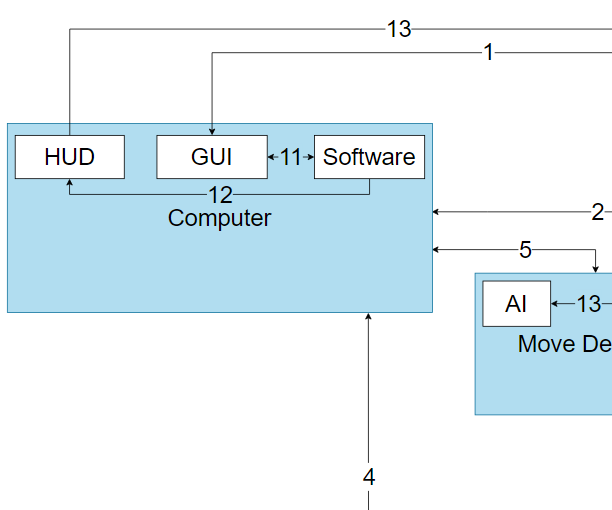
\includegraphics[width=0.80\textwidth]{images/computer_subsystems.png}
 \caption{Computer layer subsystems diagram}
\end{figure}

\subsubsection{Subsystem Hardware}
% A description of any involved hardware components for the subsystem.
A monitor connected to the computer to display game state status to the player.

% \subsubsection{Subsystem Operating System}
% A description of any operating systems required by the subsystem. removed because it is a repeat of things discussed above for the overall layer
% Linux distribution Ubuntu 22.04 LTS.

\subsubsection{Subsystem Software Dependencies}
% A description of any software dependencies (libraries, frameworks, design software for mechanical parts or circuits, etc) required by the subsystem.
This subsystem is dependent on the Software subsystem to receive information about the status of the game to display. It will also have software dependencies on GUI libraries such as PyQt5 or Tkinter.

\subsubsection{Subsystem Programming Languages}
% A description of any programming languages used by the subsystem.
The subsystem uses Python 3.10.6 as the programming language used.

\subsubsection{Subsystem Data Structures}
% A description of any classes or other data structures that are worth discussing for the subsystem. For example, data being transmitted from a microcontroller to a PC via USB should be first be assembled into packets. What is the structure of the packets?
N/A

\subsubsection{Subsystem Data Processing}
% A description of any algorithms or processing strategies that are worth discussing for the subsystem. If you are implementing a well-known algorithm, list it. If it is something unique to this project, discuss it in greater detail.
N/A



\subsection{GUI Subsystem}
% Descibe at a high level the purpose and basic design of this subsystem. Is it a piece of hardware, a class, a web service, or something else? Note that each of the subsystem items below are meant to be specific to that subystem and not a repeat of anything discussed above for the overall layer.
The Graphical User Interface (GUI) subsystem is a class that is the main interactive component between the Computer and Opponent layers. It communicates with the Software subsystem within the Computer layer for its inputs and outputs. The GUI displays buttons for the user (Opponent) to interact with. These buttons will be able to change the state of the game for purposes such as new game, restart game, and quit game. Each time the Opponent interacts with the GUI by clicking a corresponding button to a function, that button will send a mouse click signal for that button to the Software subsystem. This signals to the Software subsystem to execute the function associated with the button that is clicked. For example, if the user clicks a new game button, the software executes the processes needed to reset the state of the game and UR5 robot arm.


\subsubsection{Subsystem Hardware}
% A description of any involved hardware components for the subsystem.
A monitor connected to the computer to display the different options to the player. A mouse is also required for the player to interact with the GUI.

%\subsubsection{Subsystem Operating System}
% A description of any operating systems required by the subsystem. - removed because it is a repeat of things discussed above for the overall layer
% Linux distribution Ubuntu 22.04 LTS.

\subsubsection{Subsystem Software Dependencies}
% A description of any software dependencies (libraries, frameworks, design software for mechanical parts or circuits, etc) required by the subsystem.
This subsystem will have software dependencies on GUI libraries such as PyQt5 or Tkinter.

\subsubsection{Subsystem Programming Languages}
% A description of any programming languages used by the subsystem.
The subsystem uses Python 3.10.6 as the programming language used.

\subsubsection{Subsystem Data Structures}
% A description of any classes or other data structures that are worth discussing for the subsystem. For example, data being transmitted from a microcontroller to a PC via USB should be first be assembled into packets. What is the structure of the packets?
N/A

\subsubsection{Subsystem Data Processing}
% A description of any algorithms or processing strategies that are worth discussing for the subsystem. If you are implementing a well-known algorithm, list it. If it is something unique to this project, discuss it in greater detail.
N/A



\subsection{Software Subsystem}
% Descibe at a high level the purpose and basic design of this subsystem. Is it a piece of hardware, a class, a web service, or something else? Note that each of the subsystem items below are meant to be specific to that subystem and not a repeat of anything discussed above for the overall layer.
The Software subsystem is the main program for managing the checkers game itself and is behind the actions the UR5 Robot Arm will execute. This subsystem not only includes the source code itself, but also software packages needed for the program. The Software subsystem is responsible for handling events from the GUI. The subsystem also communicates with the UR5 robot arm through the Computer layer. The subsystem handles data on the status of the robot arm received from the robot arm itself. It also communicates to the robot arm what programmed actions it will need to perform. These actions will be determined by its interactions with the Move Decision layer which consists of the AI subsystem. The Software subsystem is also responsible for handling inputs from the Input Button/Device layer through the Computer layer.


\subsubsection{Subsystem Hardware}
% A description of any involved hardware components for the subsystem.
N/A

% \subsubsection{Subsystem Operating System}
% A description of any operating systems required by the subsystem. - removed because it is a repeat of things discussed above for the overall layer
%Linux distribution Ubuntu 22.04 LTS.

\subsubsection{Subsystem Software Dependencies}
% A description of any software dependencies (libraries, frameworks, design software for mechanical parts or circuits, etc) required by the subsystem.
The Software subsystem requires the ur\_rtde interface library to communicate with the UR5 robot arm. This library will allow us to write Python code to receive data from the UR5, and also control it. This is done using the RTDE Receive Interface API and RTDE Control Interface API from the library respectively. Documentation for the library can be found here: https://sdurobotics.gitlab.io/ur\_rtde/index.html. Controlling the UR5 includes communicating with the Move Execution layer and sending the commands to move the robot arm to a certain position. The subsystem is dependent on the Computer Vision and AI subsystems from the Move Decision layer to determine the commands it needs to send to the robot arm. It also needs this dependency to manage the checkers game and send the data required by the HUD subsystem. Moreover, it is also dependent on the GUI subsystem and Input Button/Device layer to listen to events from the player and handle them for the checkers game accordingly.


\subsubsection{Subsystem Programming Languages}
% A description of any programming languages used by the subsystem.
The subsystem uses Python 3.10.6 as the programming language used.

\subsubsection{Subsystem Data Structures}
% A description of any classes or other data structures that are worth discussing for the subsystem. For example, data being transmitted from a microcontroller to a PC via USB should be first be assembled into packets. What is the structure of the packets?
N/A

\subsubsection{Subsystem Data Processing}
% A description of any algorithms or processing strategies that are worth discussing for the subsystem. If you are implementing a well-known algorithm, list it. If it is something unique to this project, discuss it in greater detail.
N/A